% Euclidean Handout Number One
\documentclass{tufte-handout}

%\geometry{showframe}% for debugging purposes -- displays the margins

%%%% Packages to make things pretty
\usepackage{amsmath,amsthm}
\usepackage{booktabs}
\usepackage{graphicx}
\setkeys{Gin}{width=\linewidth,totalheight=\textheight,keepaspectratio}
\graphicspath{{graphics/}}
\usepackage{units}
\usepackage{fancyvrb}
\fvset{fontsize=\normalsize}
\usepackage{multicol}
\usepackage{pdfpages}

%%%% Theorem Environments
\theoremstyle{definition}
\swapnumbers
\newtheorem{problem}{Problem}[section]
\newtheorem{conjecture}[problem]{Conjecture}
\newtheorem*{definition}{Definition}
\newtheorem*{theorem}{Theorem}
\newtheorem{question}[problem]{Question}
\newtheorem{challenge}[problem]{Challenge}
\newtheorem*{postulate}{Postulate}

%%%%%


\title{Euclidean Geometry:\\An Introduction to Mathematical Work}
\author[]{Math 3600}
\date{Fall 2020}

\begin{document}

\maketitle
\begin{marginfigure}
    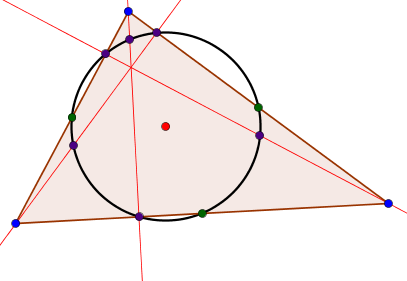
\includegraphics{NPC}
\end{marginfigure}

\setcounter{section}{3}
\section{The Geometry of Rectangles}\label{section:rectangles}

Rectangles are probably familiar to you, but to be clear we give a precise definition.
\begin{definition}\label{defn:rectangle}
A \emph{rectangle} is a quadrilateral which has all four interior angles that are right angles.
\end{definition}

Notice that the definition only speaks about angles. There is nothing at all said about the sides.
But that doesn't mean that the sides have no special properties---it is just that those properties are really theorems.
\marginnote[-40pt]{This is something many people have to get used to. It is a way in which mathematical definitions differ from common definitions in English.}

\begin{conjecture}\label{conj:rectangle-parallelogram}
Let $R$ be a rectangle. Then $R$ is a parallelogram.
\end{conjecture}

\begin{conjecture}\label{conj:rectangle-opp-sides}
Let $R$ be a rectangle. Then each pair of opposite sides of $R$ is a pair of congruent segments.
\end{conjecture}

\begin{conjecture}\label{conj:rectangle-diagonals}
The two diagonals of a rectangle are congruent and bisect each other.
\end{conjecture}

%\begin{fullwidth}
\newthought{These conjectures} describe some qualities that are common to all rectangles. Mathematicians say that these are \emph{necessary conditions} for having a rectangle.
If a figure is a rectangle, then these properties are ``necessarily'' also true. Now we shall try to go in the opposite direction.
The following conjectures are possible answers to the question, ``What kind of information does one need to claim that that our figure is a rectangle?''
Of course, we can use the definition above--that is one of the important roles of a definition, to test when we are allowed to use a word.
But what we want now are \emph{sufficient conditions}, these are conditions that allow us to conclude that our figure is a rectangle by checking something other than the definition.
%\end{fullwidth}
\marginnote[-80pt]{We will later see an example of conditions which are both
\emph{necessary} and \emph{sufficient} for something, and thus provide an example of an \emph{equivalent statement}.}


\begin{conjecture}\label{conj:opp-congruent-implies-rectangle}
Let $ABCD$ be a quadrilateral such that angles $\angle ABC$ and $\angle ADC$ are right angles.
If segments $AB$ and $CD$ are congruent, then $ABCD$ is a rectangle.
\end{conjecture}

\begin{conjecture}\label{conj:opp-parallel-implies-rectangle}
Let $ABCD$ be a quadrilateral such that angles $\angle ABC$ and $\angle ADC$ are right angles.
If segments $AB$ and $CD$ are parallel, then $ABCD$ is a rectangle.
\end{conjecture}

Notice the importance that pairs of parallel lines play in these statements.

\clearpage

\marginnote[20pt]{These results don't \emph{look} to be about rectangles.}

\begin{conjecture}[Midline Theorem] \label{conj:midline-theorem}
Let $ABC$ be a triangle, $D$ the midpoint of $AB$ and $E$ the midpoint of $AC$.
Then the line through $E$ and $D$, called a \emph{midline}, is parallel to the line through $B$ and $C$.
\end{conjecture}

\begin{conjecture}[Varignon's Theorem]\label{conj:Varignon}
Let $ABCD$ be a quadrilateral. The midpoints of the four sides are the vertices of a parallelogram.
\end{conjecture}

\begin{conjecture}[Kinda Tricky, version one] \label{conj:experiment-1}
Let $ABCD$ be a quadrilateral. If $AB$ is congruent to $CD$ and $BC$ is congruent to $AD$, then $ABCD$ is a parallelogram.
\end{conjecture}

\begin{conjecture}[Kinda Tricky, version two] \label{conj:experiment-2}
Let $ABCD$ be a quadrilateral. If $AB$ is congruent to $CD$ and angle $BCD$ is congruent to $DAB$, then $ABCD$ is a parallelogram.
\end{conjecture}


\vfill
\end{document}

%sagemathcloud={"zoom_width":100}